\documentclass{amsart}
\usepackage{tikz}
\usetikzlibrary{arrows,matrix}
\usepackage{amssymb}
\usepgflibrary{patterns}

\begin{document}

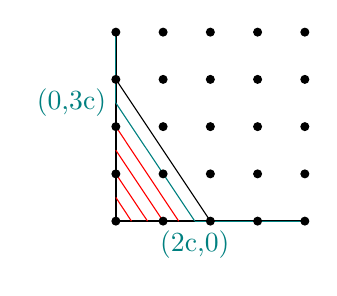
\begin{tikzpicture}[scale=0.6]
\draw[black, thick] (0,0) -- (4,0);
\draw[black, thick] (0,0)--(0,4);
\draw[black] (2,0)--(0,3);
\draw[teal] (1.67,0) node[below]{(2c,0)} --(0,2.5) node[left]{(0,3c)};
\draw[red] (1.33,0) --(0,2);
\draw[red] (1,0) --(0,1.5);
\draw[red] (.67,0) --(0,1);
\draw[red] (.33,0) --(0,.5);
\draw[teal] (1.67,0) -- (4,0);
\draw[teal] (0,2.5)--(0,4);
\foreach \x in {0,1,2,3,4}{ \node[draw,circle,inner sep=1pt,black,fill] at (\x,0) {};}
\foreach \x in {0,1,2,3,4}{ \node[draw,circle,inner sep=1pt,black,fill] at (\x,1) {};}
\foreach \x in {0,1,2,3,4}{ \node[draw,circle,inner sep=1pt,black,fill] at (\x,2) {};}
\foreach \x in {0,1,2,3,4}{ \node[draw,circle,inner sep=1pt,black,fill] at (\x,3) {};}
\foreach \x in {0,1,2,3,4}{ \node[draw,circle,inner sep=1pt,black,fill] at (\x,4) {};}

\end{tikzpicture}

\end{document}